\section{Website / front end}
Die bisherige Anzeige der Wetterdaten basiert auf Adobe Flash, was nicht von allen Browsern unterstützt wird (siehe Fachmodul-Bericht). Die neue (2014) HTML5-Spezifikation ermöglicht es dynamische Grafiken zu erzeugen, die nativ von allen Web-Browsern dargestellt werden können.



%% ###################################################################################################
%%   Unterkapitel
%% ###################################################################################################
\subsection{Nutzungsanalyse der Webseite mittels Google Analytics}
\label{subsec:googleAnalytics}
Zuerst wurden die Zugriffsdaten auf die bestehende Webseite mittels Google Analytics analysiert. Als Zeitraum wurde das gesamte Jahr 2017 gewählt. Auf der bisherigen Webseite gab es zwei Unterseiten \textit{Wetter Tourismus} und \textit{Wetter Wassersport}, die sich aber nur gering voneinander unterscheiden z.B. in der Wahl der Einheit der Windgeschwindigkeit (km/h vs. kn). Die Zugriffsdaten sind in Abbildung \ref{img:google_mobile} dargestellt. Darin lässt sich erkennen, dass der Anteil an mobilen Geräten zwischen 50\% und 80\% beträgt. Dies wiederspiegelt den Trend zum mobilen Internet und zeigt wie wichtig die mobile Version einer Webseite ist. Dies geht soweit, dass sogar die mobile Seite als Ausgangspunkt für die Entwicklung der Homepage dient nach dem Designkonzept \textit{Mobile First}.

\begin{figure}[h!]
  \fbox{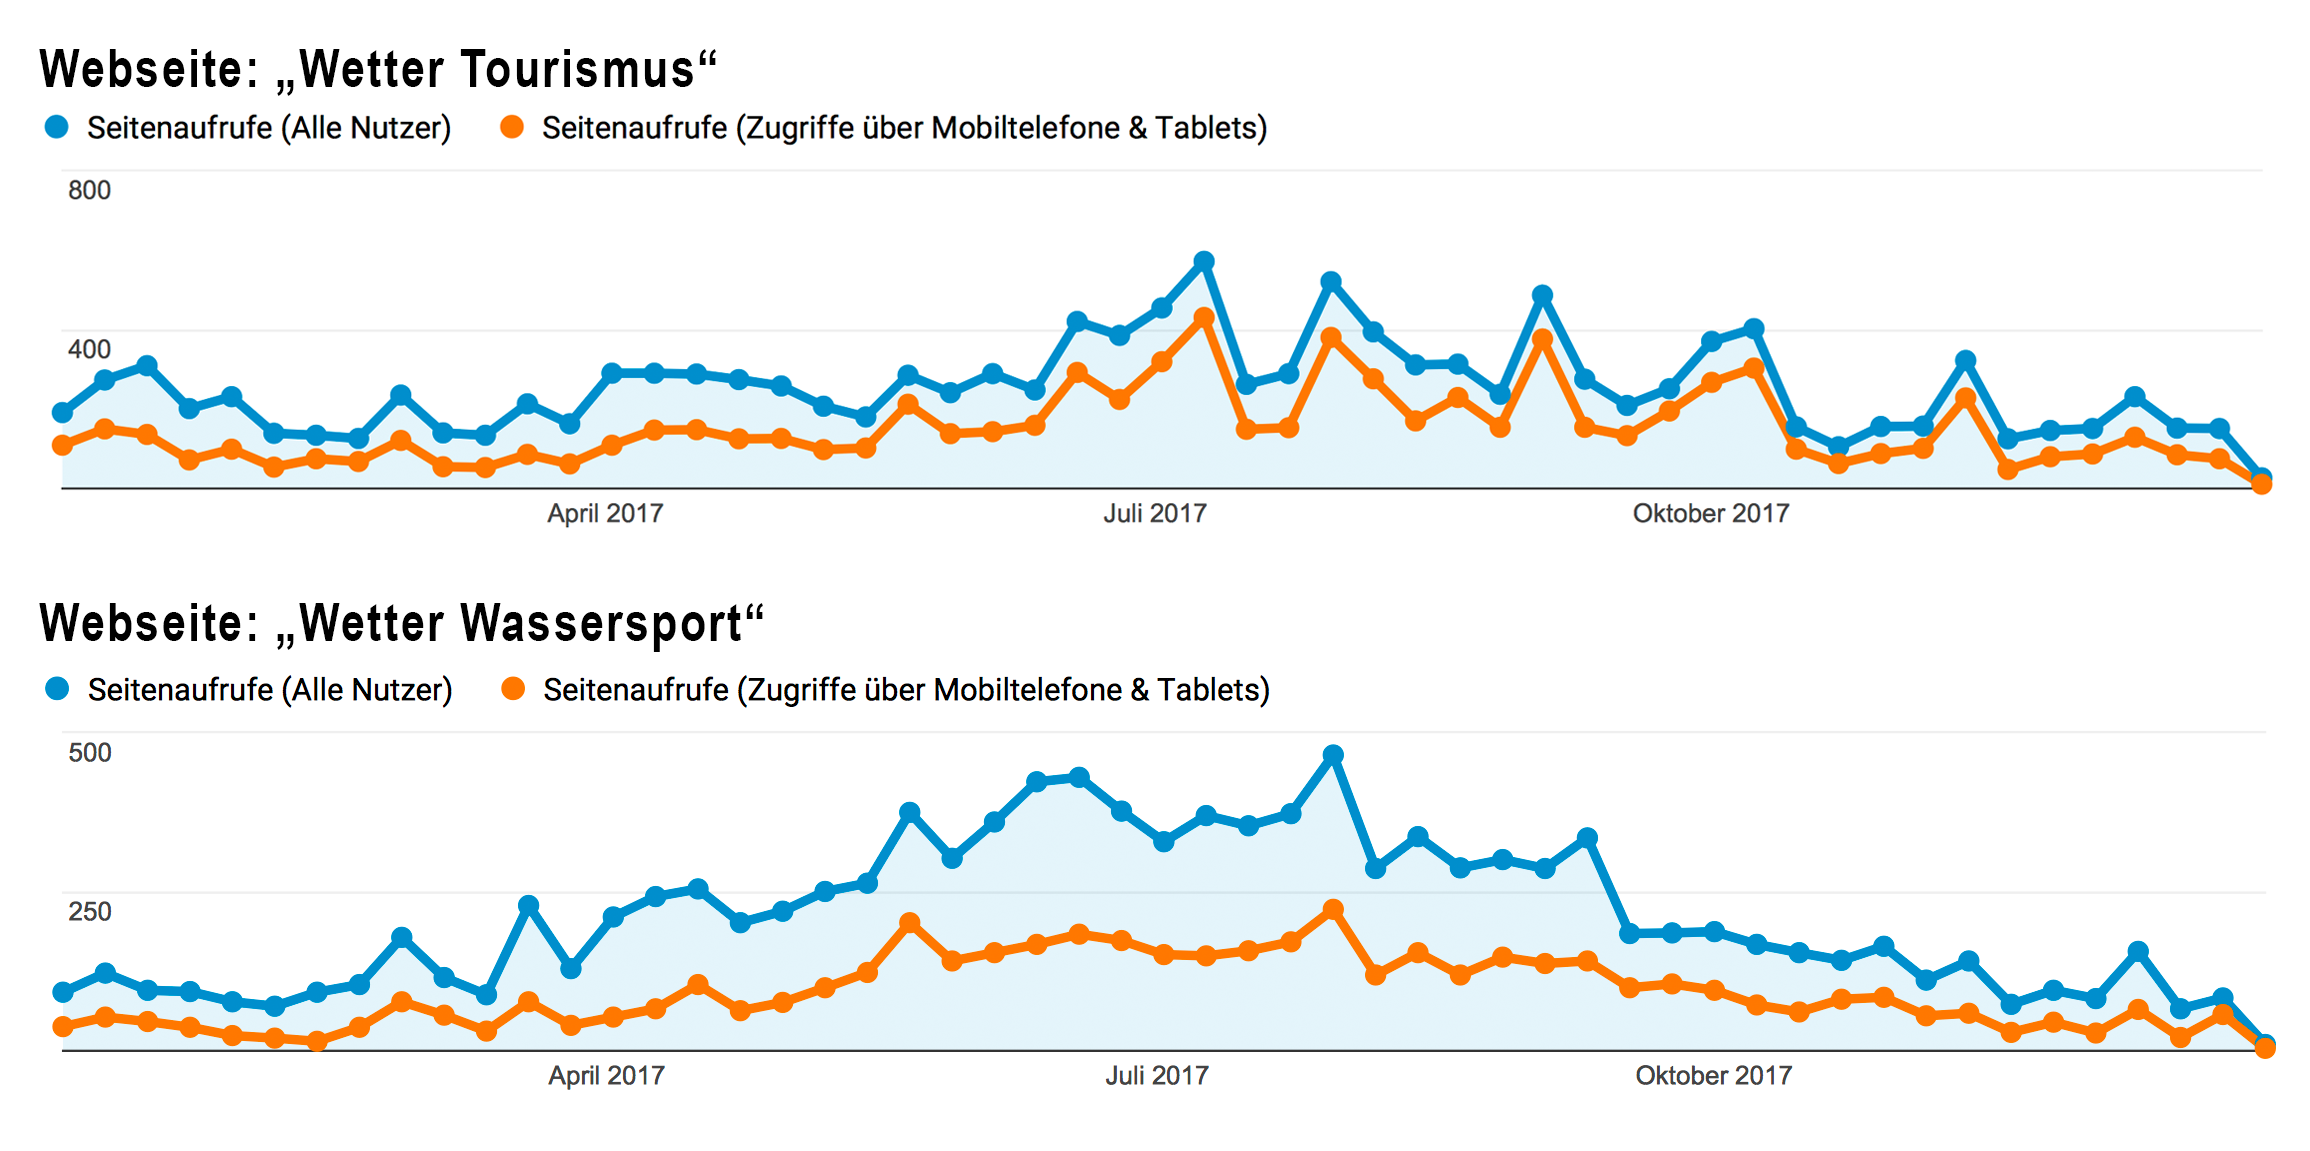
\includegraphics[width=\textwidth-2\fboxsep-2\fboxrule]{img/google_mobile}}
	\centering
	\caption{Anteil der mobilen Zugriffe auf die Wetterwebseite}
	\label{img:google_mobile}
\end{figure}

Es lässt sich ebenfalls erkennen welche Browser am häufigsten verwendet werden und welches die beliebteste Seite der Website ist, wie in Abbildung \ref{img:google_browser} dargestellt.

\begin{figure}[h!]
	\centering
	\fbox{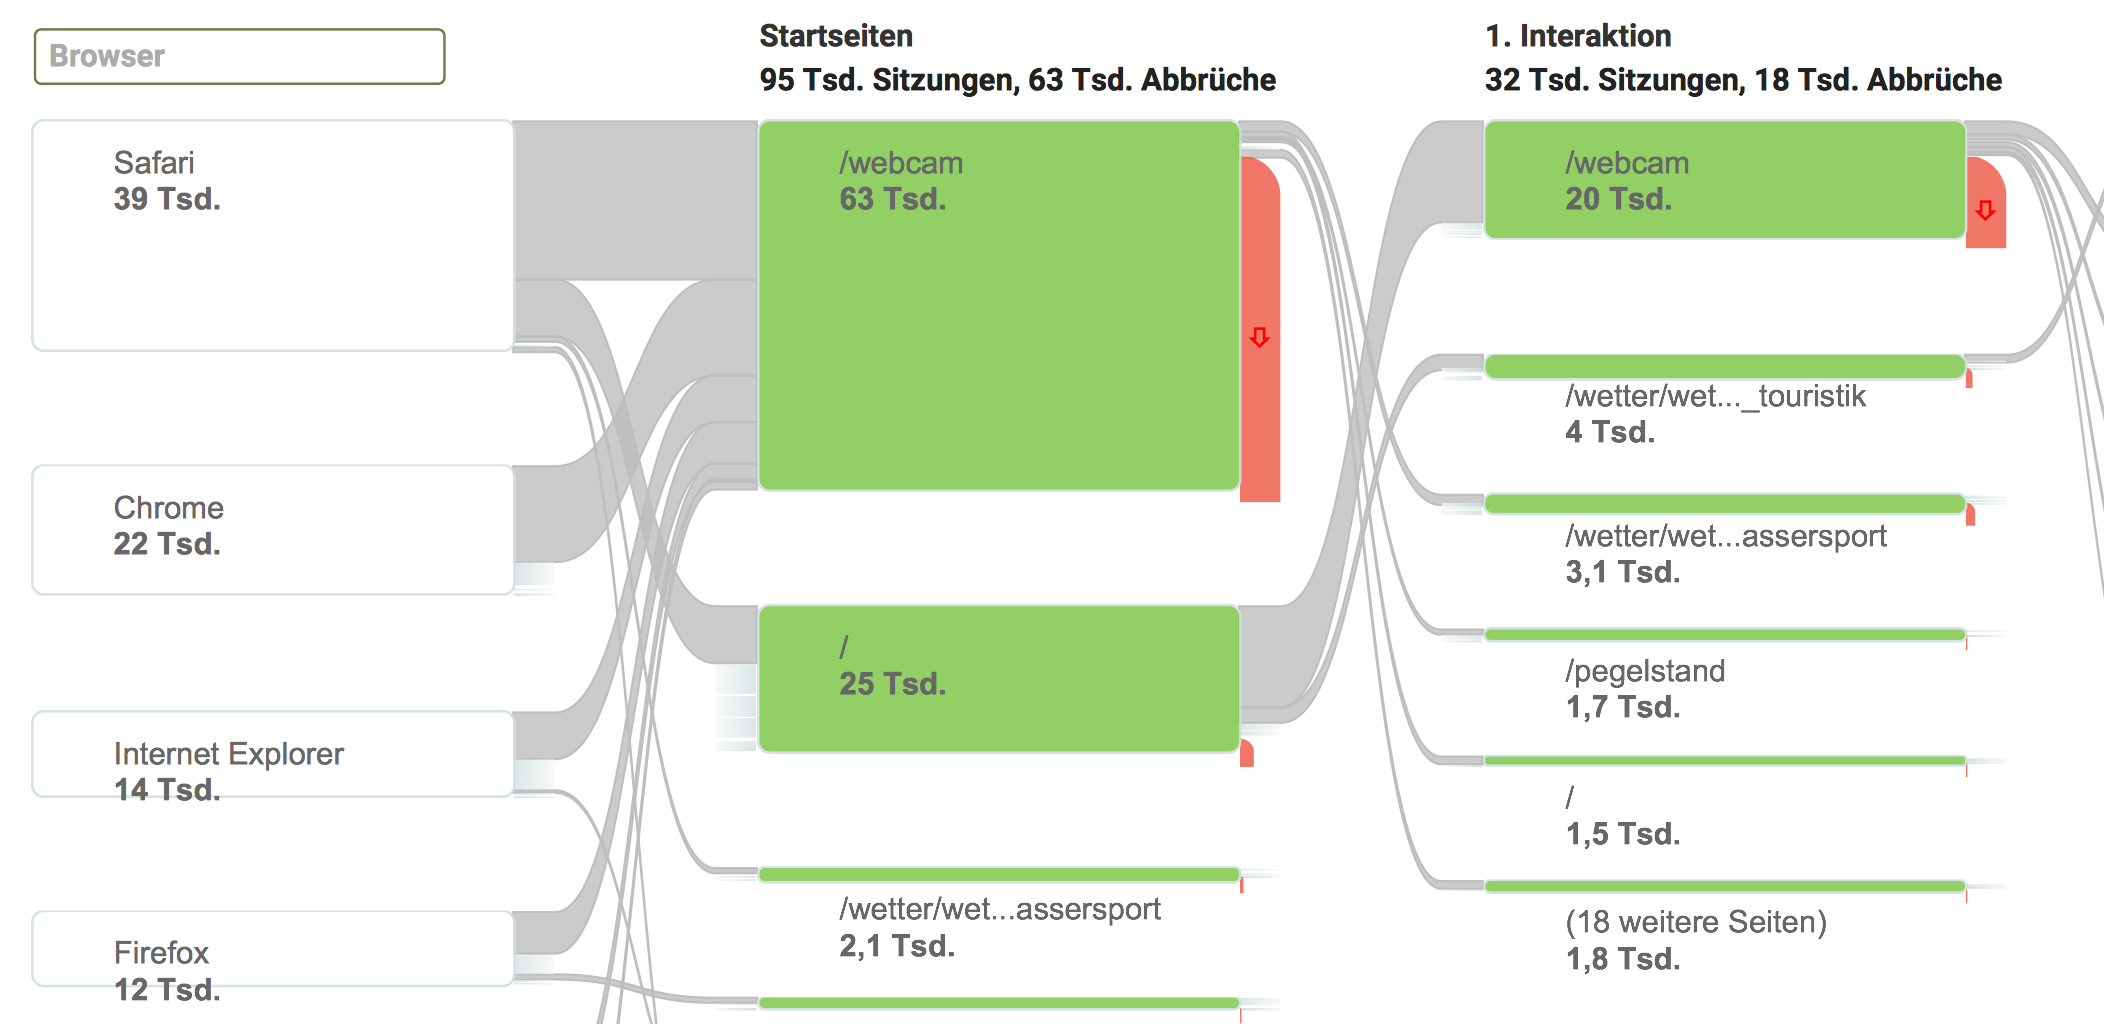
\includegraphics[width=\textwidth-2\fboxsep-2\fboxrule]{img/google_browser}}
	\caption{Verwendete Browser und Beliebtheit der Seiten}
	\label{img:google_browser}
\end{figure}



%% ###################################################################################################
%%   Unterkapitel
%% ###################################################################################################
\subsection{Konzeption der crossplattformfähigen Benutzeroberfläche}
Wie im Abschnitt \ref{subsec:googleAnalytics} aufgezeigt werden bereits heute 50\% bis 80\% der Aufrufe von mobilen Geräten ausgeführt, Tendenz steigend. Es ist deshalb naheliegend das mobile Design als Startpunkt zu verwenden. Diese Vorgehensweise nennt sich \textit{Mobile First}. Es ist ein Designkonzept, das von Luke Wroblewski 2009 das erste Mal vorgeschlagen wurde. Die optimale Darstellung einer Website auf mobilen Endgeräten hat dabei oberste Priorität. Bei Mobile First beginnt der Designer mit dem Mobile-Design und arbeitet sich dann schrittweise zur grösseren Desktop-Version vor. Die \flqq Mobile Web Best Practices\frqq \footnote{ \url{https://www.w3.org/TR/mobile-bp}} des W3C empfiehlt zudem, dass sämtliche Informationen, die in der Desktop-Version zur Verfügung stehen, auch von der mobilen Seite aufgerufen werden können. Dieser Grundsatz nennt sich \textit{One Web Design}.

\begin{figure}[h!]
  \fbox{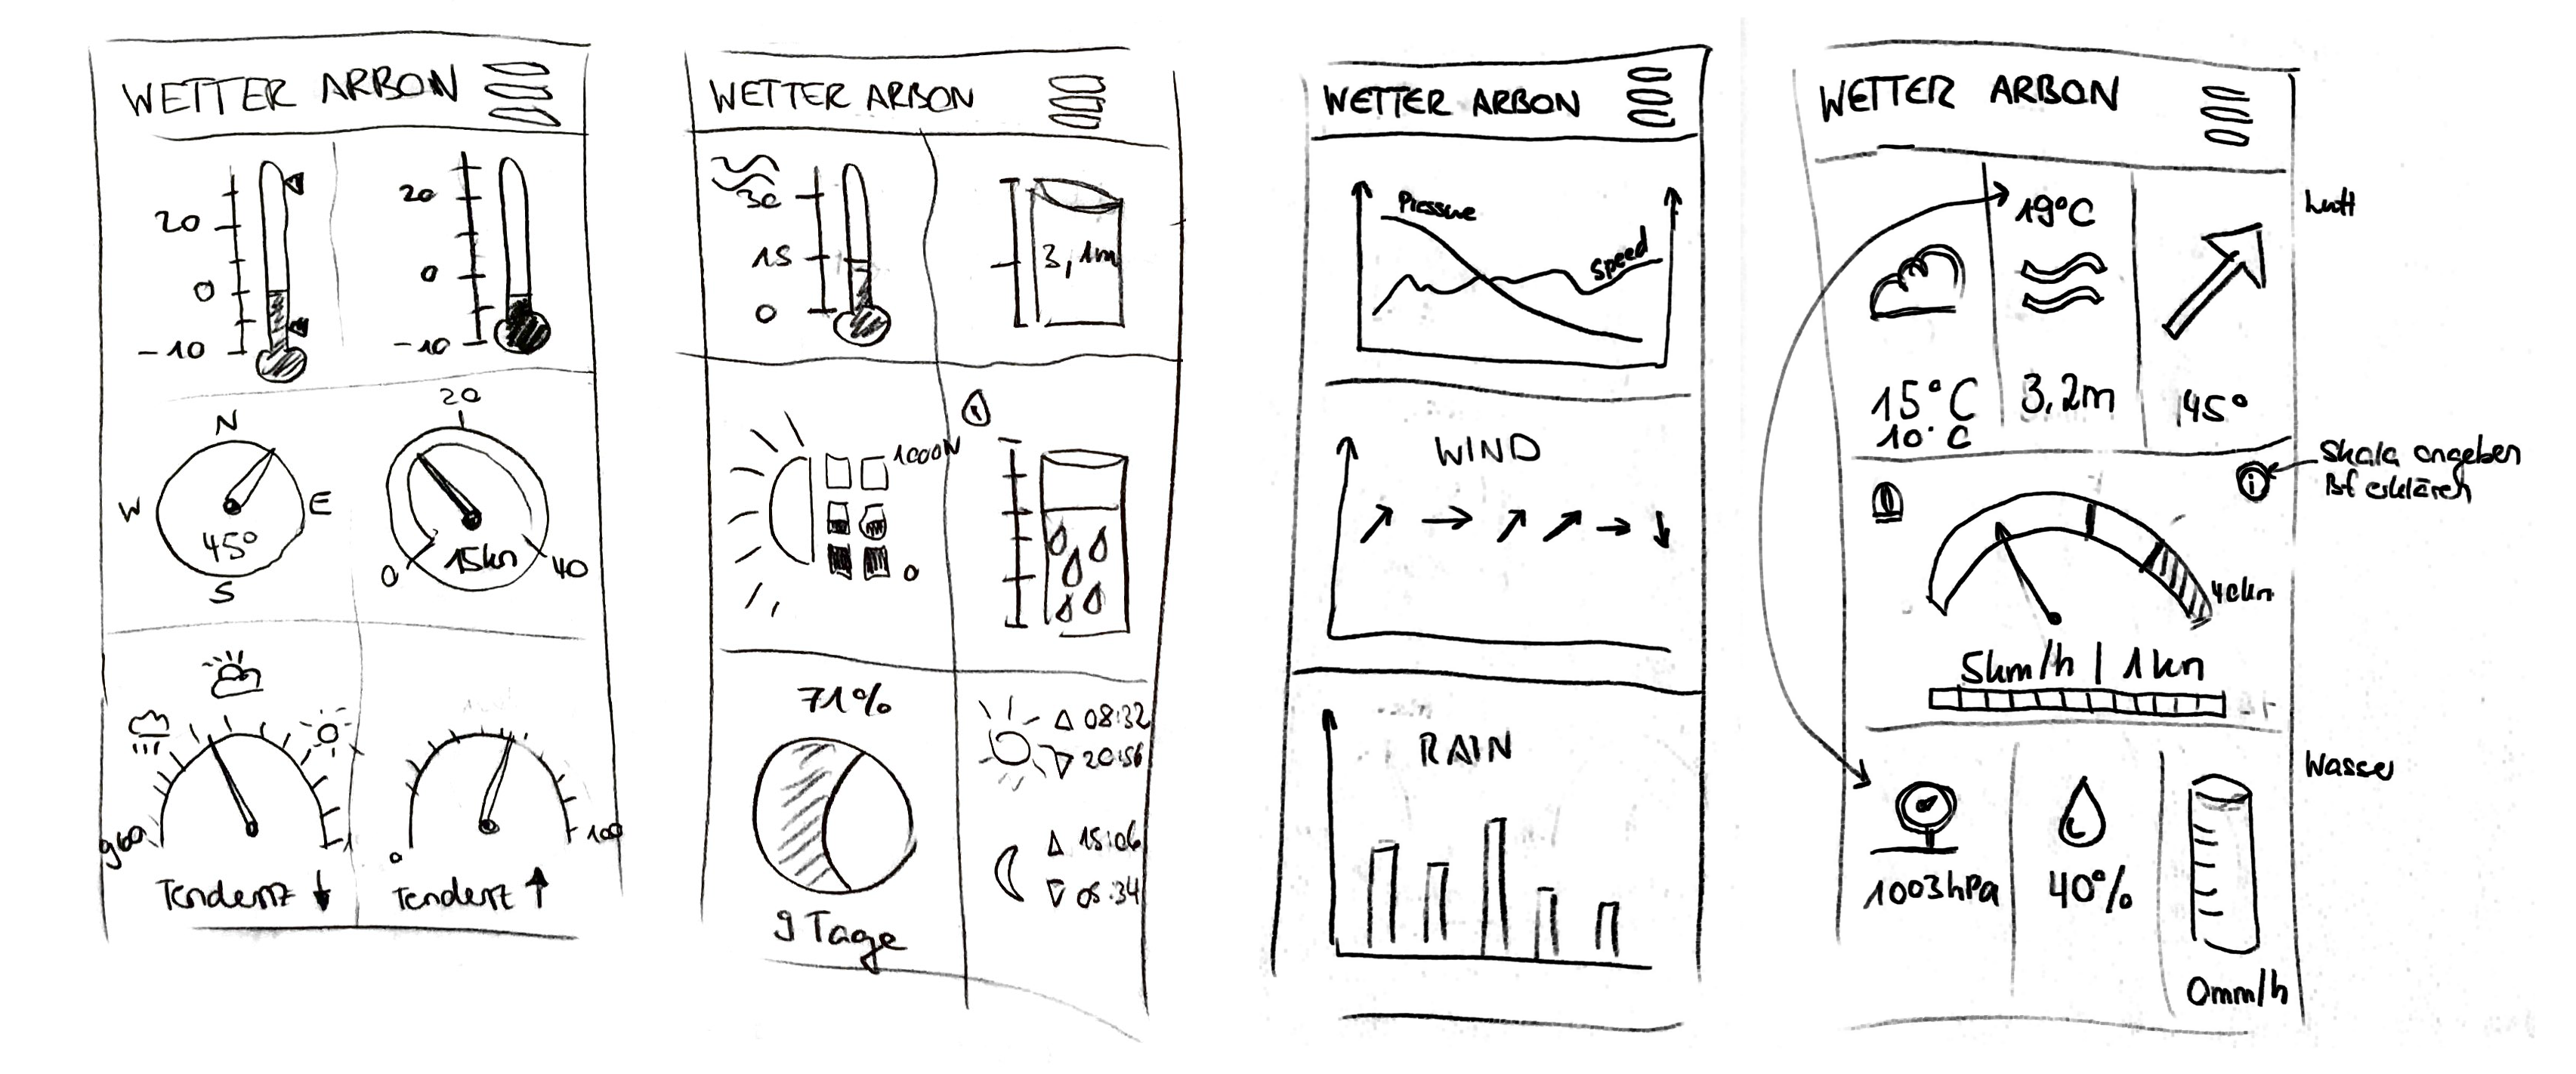
\includegraphics[width=\textwidth-2\fboxsep-2\fboxrule]{img/scribbles}}
	\centering
	\caption{Erste Designentwürfe nach dem Mobile First Prinzip}
	\label{img:scribbles}
\end{figure}

Beim Erstellen der ersten Designentwürfe, wie in Abbildung \ref{img:scribbles}, dargestellt, stellte sich schnell heraus, dass die einfachste Möglichkeit die Daten auf allen Bildschirmgrössen darzustellenzu können, darin besteht, die Informationen in kleine logische Blöcke zu unterteilen. Diese Blöcke können dann verschieden angeordnet werden. Dieses Kachel-Design ist eine gängiges Prinzip um das Gestaltungsgesetz der Zusammengehörigkeit umzusetzen und eignet sich hervorradend im Zusammenhang mit dem Grid-Konezpt des responsive Designs, welches im Abschnitt \ref{subsec:responsiveFactors} erläutert wird.


\subsubsection{W3.css als Layout-Framework}
Sämtliche Artefakte unserer Arbeit sollen möglichst einfach gehalten werden. Für die Gestaltung der Benutzeroberfläche haben wir uns deshalb entschlossen ein CSS-Framework zu benutzen. Dieses soll möglichst einfach und intuitiv zu bedienen sein, das Kachel-Design (auch Card-Design genannt) unterstützen, eine ausführliche Dokumentation aufweisen und eine geringe Dateigrösse haben. Wir haben drei verschieden CSS-Frameworks evaluiert und bewertet. Das Resultat ist in Tabelle  \ref{table:css-framework} ersichtlich.

\begin{table}[htb!]
\setlength\extrarowheight{3pt} % for a more "open" look
\begin{tabularx}{\textwidth}{|>{\RaggedRight\hspace{0pt}}p{4cm}||X|X|X|}

\hline
& \bfseries\large \href{https://www.w3schools.com/w3css/default.asp}{W3.css}
& \bfseries\large \href{https://purecss.io/start/}{Pure.css}
& \bfseries\large \href{http://getbootstrap.com/docs/4.1/getting-started/introduction/}{Bootstrap}\\

\hline
\textbf{Grid Design}
& ++
& ++
& ++ \\

\hline
\textbf{Footprint}
& 23 kB
& 14 kB
& 141 kB \\

\hline
\textbf{Usability}
& ++
& +
& + \\

\hline
\textbf{Card-Design}
& +
& -
& ++ \\

\hline
\textbf{Dokumentation}
& +++
& 0
& ++ \\

\hline
\textbf{Cross-Browser}
& ++
& ++
& +++ \\

\hline
\textbf{Funktionsumfang}
& +
& 0
& ++ \\

\hline
\end{tabularx}
\caption{Beurteilungsmatrix der evaluierten css-Frameworks}
\label{table:css-framework} % label muss NACH caption stehen!!!!
\end{table}

\noindent
Als Sieger stellt sich das W3.css-Framework heraus, da es den besten Kompromiss zwischen Dateigrösse und Funktionsumfang bietet. Zumdem weist es eine hervorragende Dokumentation auf.


\subsubsection{Responsive Design}
\label{subsec:responsiveFactors}
Die Benutzeroberfläche muss Cross-Plattform-fähig sein d.h. die Darstellung muss sich je nach Bildschirmgrösse automatisch anpassen. Man nennt dies \textit{Responsive Design}. Die Idee des Responsive Web Design wurde 2010 von Ethan Marcotte in einem Artikel\footnote{ \url{http://alistapart.com/article/responsive-web-design}} des Magazins \textit{A List Apart} veröffentlicht. Hintergrund war, dass man nicht für jedes neue Gerät eine eigene Webseite erstellen wollte. Marcotte schreibt von drei Faktoren, die ein responsive Design benötigt: Fluid grids, flexible images und media queries. Fluid grids bedeutet, dass sich die Anordnung der Elemente dynamisch der Bildschirmgrösse anpasst. Flexible Bilder haben keine feste Grösse sondern nutzen den ihnen zu Verfügung stehenden Platz optimal aus und die Media queries sind die technische Basis für die beiden oberen Anforderungen.

\begin{figure}[h!]
  \fbox{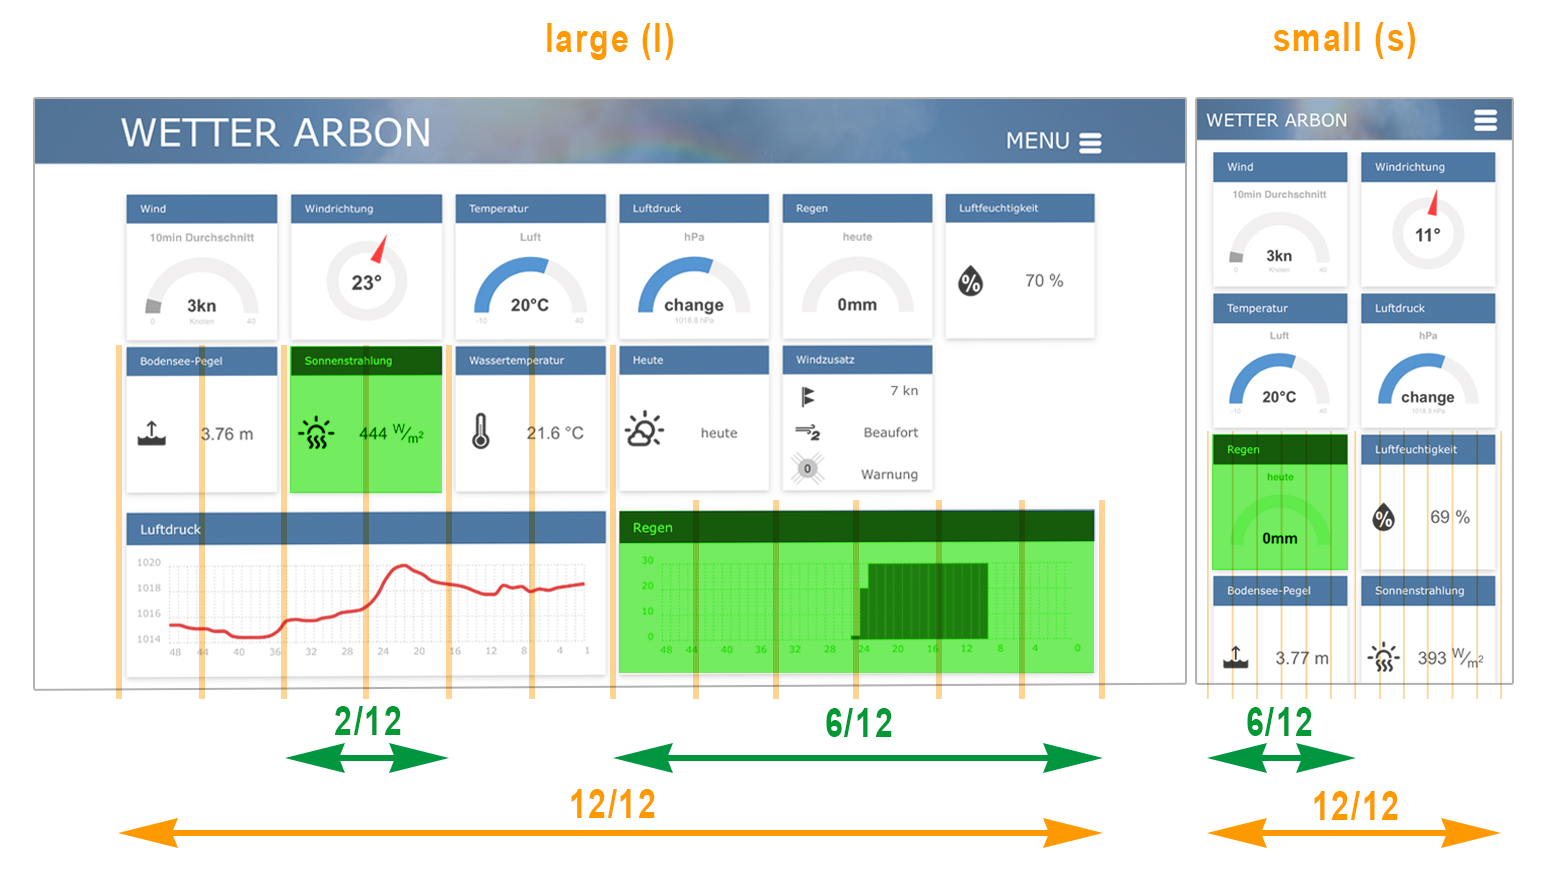
\includegraphics[width=\textwidth-2\fboxsep-2\fboxrule]{img/kacheln2}}
	\centering
	\caption{Anordnung der Kacheln auf grossen und kleinen Bildschirmen}
	\label{img:kacheln2}
\end{figure}

\noindent
Das Konezt des Grid-View teilt den Bildschirm in zwölf Spalten ein. Über eine media-Query fragt die Webseite die Grösse des Bildschirms ab. Es gibt drei Kategorien small, medium, large, deren Grenzen folgendermassen festgelegt sind:

\begin{itemize}
\item Small: s $\leq$ 600px (z.B. iPhone Hochformat)
\item Medium: 600px < m $\leq$ 992px (z.B. iPhopne Querformat, iPad Hochformat)
\item Large: 993px < l (z.B. Desktop)
\end{itemize}

\noindent
Im css-Framework kann nun sehr einfach definiert werden wie sich die Kacheln bei diesen drei Bildschirmkategorien verhalten sollen. Die Kacheln der aktuellen Daten sind auf grossen (large) Bildschirmen \nicefrac{2}{12}, auf mittleren Bildschirmen \nicefrac{3}{12} und auf kleinen Bildschirmen \nicefrac{6}{12} breit. Bei den Datenverläufen werden bei mittleren und grossen Bildschirmen zwei nebeneinander dargestellt, bei kleinen Bildschirmen alle untereinander.

\begin{lstlisting}[label=lst:kacheln,caption=Konfiguration der Anzahl Kacheln abhähngig von der Bildschirmgrösse, language=HTML5, style=htmlcssjs]
<!-- Aktuelle Daten -->
<div class="w3-col l2 m3 s6">
	<div class="w3-card">...</div>
</div>

<!-- Datenverlauf -->
<div class="l6 m6 s12">
	<div class="w3-card">...</div>
</div>
\end{lstlisting}

%% ###################################################################################################
%%   Unterkapitel
%% ###################################################################################################
\subsection{Grafische Darstellung der aktuellen Wetterdaten}
Die Anzeigeelemente für die aktuellen Messwerte sollen ebenfalls mit Hilfe eines Frameworks erstellt werden. Damit die Grafiken optimal mit dem responsive Layout zusammenspielen, müssen sie ein flexibles Layout aufweisen d.h. ihre Grösse dem vorhanden Platz anpassen. Am Besten nicht nur beim Aufrufen der Seite, sondern auch beim Ändern der Fenstergrösse. Zudem muss es einfach möglich sein die Werte zu aktualisieren.

Die Anzeige sollte möglichst ein klares Design aufweisen aber trotzdem individuell anpassbar sein. Ein sehr einfaches JavaScript-Framework ist \textit{JustGage}\footnote{ \url{http://justgage.com}}. Die Grafiken lassen sich über eine JavaScript-Datei konfigurieren, die Grafiken selbst sind im svg-Format und somit von praktisch allen Browsern darstellbar. JustGage basiert auf der \textit{Raphaël}\footnote{ \url{http://dmitrybaranovskiy.github.io/raphael/}}—JavaScript Bibliothek.

\begin{figure}[h!]
  \fbox{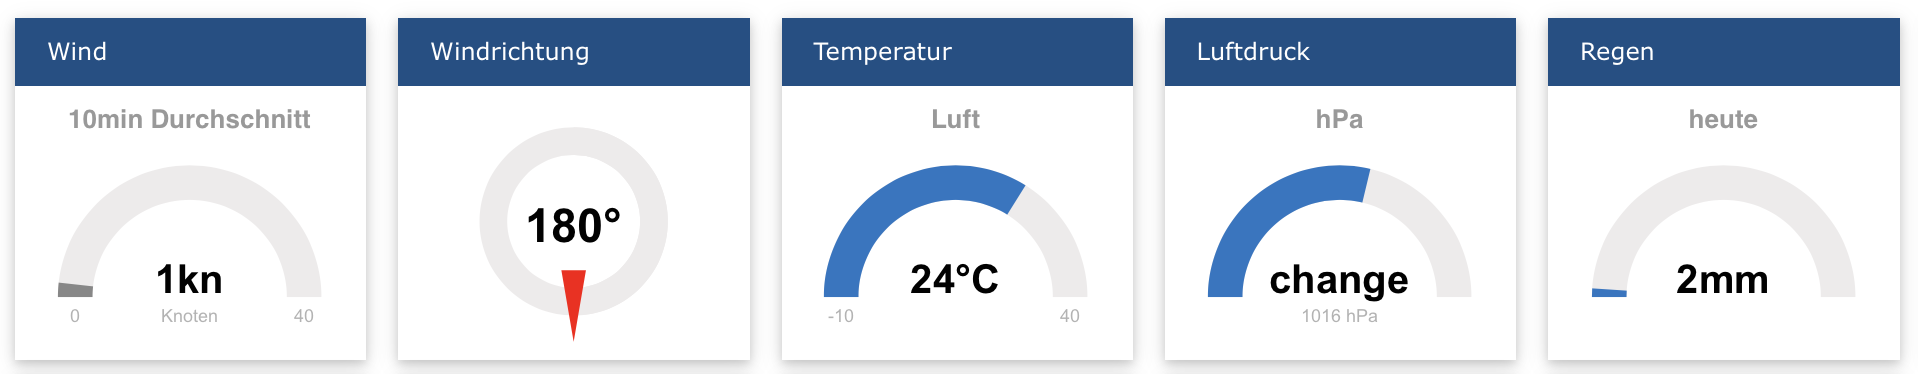
\includegraphics[width=\textwidth-2\fboxsep-2\fboxrule]{img/gauges}}
	\centering
	\caption{Anzeigelemente mit Justgage/Raphaël}
	\label{img:gauges}
\end{figure}

Raphaël ist eine kleine JavaScript-Bibliothek, die Ihnen die Arbeit mit Vektorgrafiken im Web erleichtern soll. Wenn Sie z.B. Ihr eigenes Diagramm oder Bildausschnitt erstellen und das Widget drehen möchten, können Sie dies einfach und bequem mit dieser Bibliothek erreichen. Raphaël verwendet die SVG W3C Recommendation und VML als Grundlage für die Erstellung von Grafiken. Dies bedeutet, dass jedes grafische Objekt, das Sie erstellen, auch ein DOM-Objekt ist, so dass Sie JavaScript-Ereignisbehandler anhängen oder später ändern können. Raphaëls Ziel ist es, einen Adapter zur Verfügung zu stellen, der das Zeichnen von Vektorgrafiken browserübergreifend und einfach macht.


\begin{lstlisting}[label=lst:gaugeJS,caption=Konfiguration der Gauge, language=JavaScript,mathescape, style=htmlcssjs]
var temperature_gauge = new JustGage({
  id:     temperature_gauge,
  value:  initialValues.v1.data.temperature.value,
  min:    -10,
  max:    40,
  symbol: C,
  title:  Luft
});
\end{lstlisting}

Um die Grafik anzuzeigen muss nur ein DIV mit der selben ID auf der Webseite erstellt werden wie in Listing \ref{lst:gaugeHTML} dargestellt.

\begin{lstlisting}[label=lst:gaugeHTML,caption=Container für die SVG-Grafik (Gauge), language=HTML5, style=htmlcssjs]
<!-- Lufttemperatur -->
<div class="w3-cell w3-col l2 m3 s6">
  <div class="w3-card">
    <div class="w3-container">
      <p>Temperatur</p>
    </div>
    <div id="temperature_gauge" class="gauge"></div>
  </div>
</div>
\end{lstlisting}

Die Messwerte sind einerseits über den Titel beschrieben, sie enthalten aber zusätzlich ein passendes Icons. Es wurde eine Icon-Bibliothek gewählt, die möglichst alle benötigen Icons enthält, die kostenlos ist, und deren Grafiken im svg-Format vorliegen. Als geeignet schienen die \textit{Weahter Icons}\footnote{\url{http://erikflowers.github.io/weather-icons/}} von Erik Flowers.


\begin{figure}[h!]
  \fbox{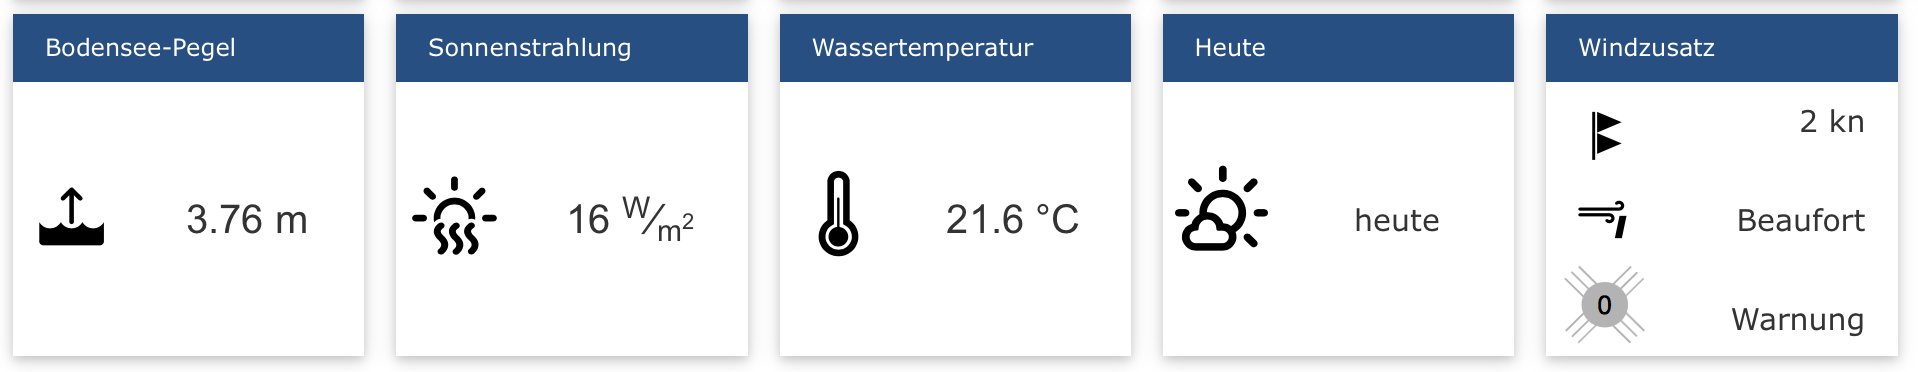
\includegraphics[width=\textwidth-2\fboxsep-2\fboxrule]{img/icons}}
	\centering
	\caption{Icons aus der Weather Icons Bibliothek}
	\label{img:icons}
\end{figure}





%% ###################################################################################################
%%   Unterkapitel
%% ###################################################################################################
\subsection{Grafische Darstellung der Wetterdatenverläufe}
Die Wetterverlaufsdarstellung soll einen Überblick über die Wettertendenz der letzten beiden Tage liefern. Die Samplerate beträgt 1h, d.h. die Daten werden aus der Tabelle der historischen Werte abgerufen.

\begin{figure}[h!]
  \fbox{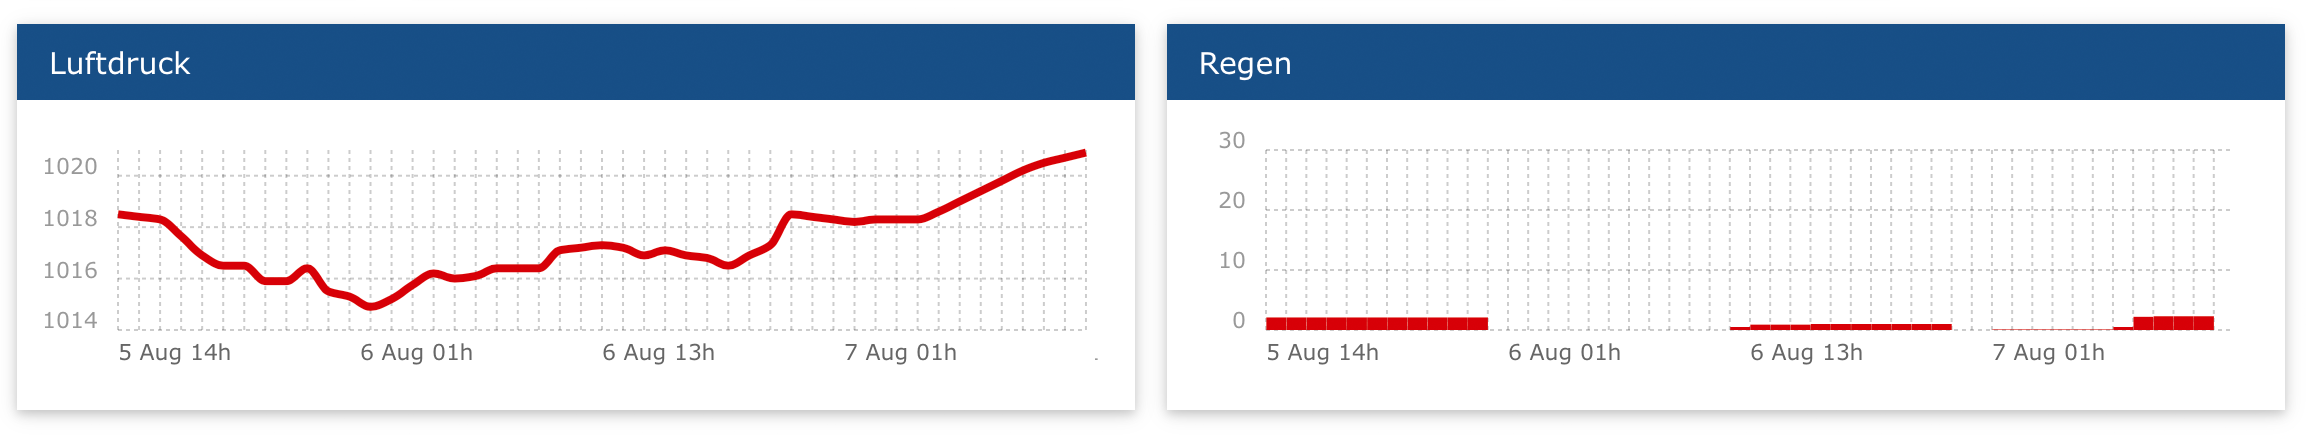
\includegraphics[width=\textwidth-2\fboxsep-2\fboxrule]{img/charts}}
	\centering
	\caption{Verlaufsdiagramm mit chartist.js}
	\label{img:charts}
\end{figure}



\subsubsection{Auswahl des JS-Frameworks}
Für die Darstellung der Messwertverläufe soll ebenfalls auf eine Bibliothek zurückgegriffen werden. Als erstes wurden js-Bibliotheken gesucht, die ein ansprechendes Design aufweisen. Übrig geblieben sind die in Tabelle \ref{table:js-framework} aufgeführten drei js-Bibliotheken. Diese wurden auf ihre Eignung geprüft. Zwingend mussten die Grafiken im SVG-Dateiformat vorliegen, sodass die Cross-Browser-Kompatiblität und das responsive Verhalten sichergestellt ist. Die Daten sollten zudem als JSON übergeben werden können. D3 ist zwar DIE js-Bibliothek wenn es um Visualisierungen im Web geht, hat aber keine vorgefertigten Diagramme und benötigt entsprechend viel Aufwand und Einarbeitungszeit, was wir explizit nicht möchten.

\begin{table}[htb!]
\setlength\extrarowheight{3pt} % for a more "open" look
\begin{tabularx}{\textwidth}{|>{\RaggedRight\hspace{0pt}}p{3.5cm}||X|X|X|}

\hline
& \bfseries\large \href{https://gionkunz.github.io/chartist-js/index.html}{chartist.js}
& \bfseries\large \href{https://www.fusioncharts.com}{Fusion Charts}
& \bfseries\large \href{https://developers.google.com/chart/}{Google Charts}\\

\hline
\textbf{Footprint}
& 10 kB
& >1000 kB
& 110 kB \\

\hline
\textbf{Barrierefrei}
& +
& 0
& + \\

\hline
\textbf{Anpassbarkeit}
& ++
& +++
& ++ \\

\hline
\textbf{Dokumentation}
& +++
& +++
& ++ \\

\hline
\textbf{Kostenlos}
& +
& --
& + \\

\hline
\textbf{Funktionsumfang}
& ++
& +++
& + \\

\hline
\end{tabularx}
\caption{Beurteilungsmatrix der evaluierten js-Frameworks}
\label{table:js-framework} % label muss NACH caption stehen!!!!
\end{table}

\noindent
Chartist.js stellte den besten Kompromiss zwischen Funktionsumfang, Einfachheit und Dokumentation dar. Insbesondere die Dateigrösse war ausschlaggebend, da die Webseite, wie in Abschnitt \ref{subsec:googleAnalytics} erklärt, primär von mobilen Nutzer genutz wird.

% Code-Beispiel
\begin{lstlisting}[label=lst:charts,caption=Konfiguration der Verlaufsdiagramme, language=HTML5, style=htmlcssjs]
//Luftdruck
var Barometer = {
  labels: [48,...,1],
  series: [dataBarometerHistoric]
};
new Chartist.Line('#air-chart', Barometer);

//Regen
var Rain = {
	labels: [48,...,1],
	series: [dataRainHistoric]
};
var options = {
low: 0,
high: 30,
};
new Chartist.Bar('#rain-chart', Rain, options);
\end{lstlisting}
\ \\


Zur Verlaufsdarstellung wird primär das Linien- und Balkendiagramm verwendet, wie in Abbildung \ref{img:charts} aufgezeigt. Für jede Grafik wurde entschieden ob eine automatische Y-Achs-Skalierung sinnvoll ist oder nicht. Bei der Windgeschwindigkeit und beim Pegel wurd bewusst eine fixe Skalierung verwendet, damit auf den ersten Blick klar ist, ob der Wert eher hoch oder eher tief ist. Beim Luftdruck hingegen ist die Tendenz wichtig, weshalb möchglichst die gesamte Höhe des Diagramms genutzer werden soll. Es wird daher eine automaitsche Y-Achs-Skalierung verwendet. Die Konfiguration erfolgt in einem einfach JS-File wie in Listing Listing \ref{lst:charts}  dargestellt. Unter \textit{options} kann die y-Achse auf die gewünschten Werte fixiert werden.\newline


\subsubsection{Anzeige der Windrichtung}
\Diskussionspunkt{- Windrichtungsverlauf -> geht nicht mit chartist -> welche andere js-Bibliothek?}\newline



\subsubsection{Vergleich Prognose/Ist Windgeschwindigkeit}

Die Messdaten der Wetterstation werden mit zwei Vorhersagediensten verglichen. Dabei wird jeweils die Eintages-Vorschau und die Dreitagesvorschau betrachtet.
Die Vorhersagedaten werden von den Anbietern nur in die Zukunft angezeigt d.h. wie die Vorhersage von gestern war ist nicht mehr ersichtlich. Aus diesem Grund müssen wir die Vorhersagedaten abgreifen und in unsere Datenbank speichern. Die Vorhersagen haben häufig einen Intervall von drei Stunden. Wir erstellen somit ein Skript, welche alle drei Stunden die Daten abfragt und speichert.

Die Darstellung von Vorhersage und Messresultaten erfolgt in einem Graphen, der den heutigen Tag, links davon die letzten 14 Tage und rechts davon die nächsten drei Tage anzeigt. Pro Anbieter und Prognoseart (1Tag bzw. 3 Tage) wird ein eigener Graph erstellt.

Diese Vergleiche werden aus reinem Interesse der IG erstellt und stellen keinen Service der IG dar. Die Wetterstation ist zudem windtechnisch eher an einem ungünstigen Ort platziert (Bucht), sodass die Messwerte nicht für den ganzen See representativ sind.
Aus diesen Gründen wird die Webseite zwar veröffentlicht, aber kein Link dazu auf der Webseite zur Verfügung gestellt.

Für den Prognoseanbieter haben wir uns für Openweathermap und windfinder entschieden. OWM bietet eine kostenlose Web-API. Windfinder ist eines der beliebtesten Seglertools, bietet aber keine API an. Dies Daten müssen somit aus der Windfinder-Webseite extrahiert werden.

Für die Darstellung der aktuellen Windgeschwindigkeit verwenden wir den Mittelwert der drei Werte aus der Stundenwert-Datenbank.

Openweathermap scheint sehr ungenaue Windvorhersagen zu liefern.

\Diskussionspunkt{-> Bild mit Vergleich von Messwerten, Vorhersage Windfinder und Vorhersage Openweathermap}\newline

% API
% Crawlers
Windfinder bietet keine API an nur Windget

Für die Windvorhersage haben wir zwei Anbieter ausgewählt:

Windfinder
Openweathermap
Ziel ist, dass wir die Vorhersagedaten der beiden Anbieter abrufen und bei uns in der Datenbank speichern. Openweathermap bietet eine kostenlose Web-API an, windfinder leider nicht. Wir rufen die Daten über ein Python-Skritp ab. Da Windfinder keine API anbietet, müssen die Daten aus der Webseite extrahiert werden. Ein mögliches Tool dazu ist BeautifulSoup.

Für den Vergleich der Windvorhersagedaten hatten wir zwei Dienstleister ausgewählt:

Windfinder
Openweathermap
Von beiden haben wir während den letzten zwei Wochen die Windvorhersagedaten ausgelesen und in unsere Datenbank gespeicher. Es hat sich allerdings gezeigt, dass die Vorhersagedaten von Openweathermap nicht brauchbar sind. Die Vorhersage schwankt konstant zwischen 0kn und 1kn. Wir haben uns deshalb auf die Vorhersage von Windfinder konzentriert und arbeiten mit diesen Daten weiter.

Wie oben beschrieben müssen wir die Vorhersagedaten von Windfinder aus der Webseite extrahieren. Lokal funktioniert die Abfrage. Auf dem Hostpoint-Server haben wir aber die Berechtigung nicht um BeautifulSoup zu installieren. Lösungsvorschläge sind erwünscht.

%View
SELECT ABS(TIMEDIFF("2018-07-01 23:00", "2018-07-02 00:30")); Resultat: 13'000


\begin{lstlisting}[label=lst:viewForecast,caption=Erzeugung der VIEW für den Forecast-Vergleich, language=SQL, style=htmlcssjs]
SELECT *
FROM 'tblcompwindfinder'
WHERE
(datetime + interval 3 day) <= now() #heute vor drei Tagen
AND
abs(timediff(datetime,now())) <= 13000) #innerhalb +/- 1.5h
ORDER BY datetime DESC
LIMIT 3
\end{lstlisting}

%% ###################################################################################################
%%   Unterkapitel
%% ###################################################################################################
\subsection{Anzeige der aktuellen Sturmwarn-Situation}
\label{subsec:sturmwarnung}

% was ist der Sturmwarndienst und wie werden die verschiedenen Stufen dargestellt
Auf dem Bodensee gibt es einen Sturmwarndienst, der die Schiffsführer vor aufkommendem Sturm warnen soll. Der Sturmwarndienst wird vom Deutschen Wetterdienst in Zusammenarbeit mit MeteoSchweiz betrieben. Rund um den Bodensee sind dafür über 60 Sturmwarnleuchten installiert (Abbildung \ref{img:sturm2}). Es wird unterschieden zwischen \textit{Starkwindwarnung} und \textit{Sturmwarnung}. Erstere weist auf auf starke Windböen zwischen 25 Knoten und 33 Knoten hin und wird durch Aufleuchten von orangefarbigen Blinklichtern mit ca. 40 orangefarbigen Blitzen pro Minute an den Sturmwarnleuchten signalisiert. Letzere kündigt das Auftreten von Windböen von 34 Knoten und mehr an und wird durch Aufleuchten von orangefarbigen Blinklichtern mit ca. 90 orangefarbigen Blitzen pro Minute an den Sturmwarnleuchten signalisiert (gemäss Anlage B der Bodensee-Schifffahrts-Ordnung\footnote{ \url{https://www.admin.ch/opc/de/classified-compilation/19760005/index.html}}, BSO).

\begin{figure}[h!]
	\centering
  \fbox{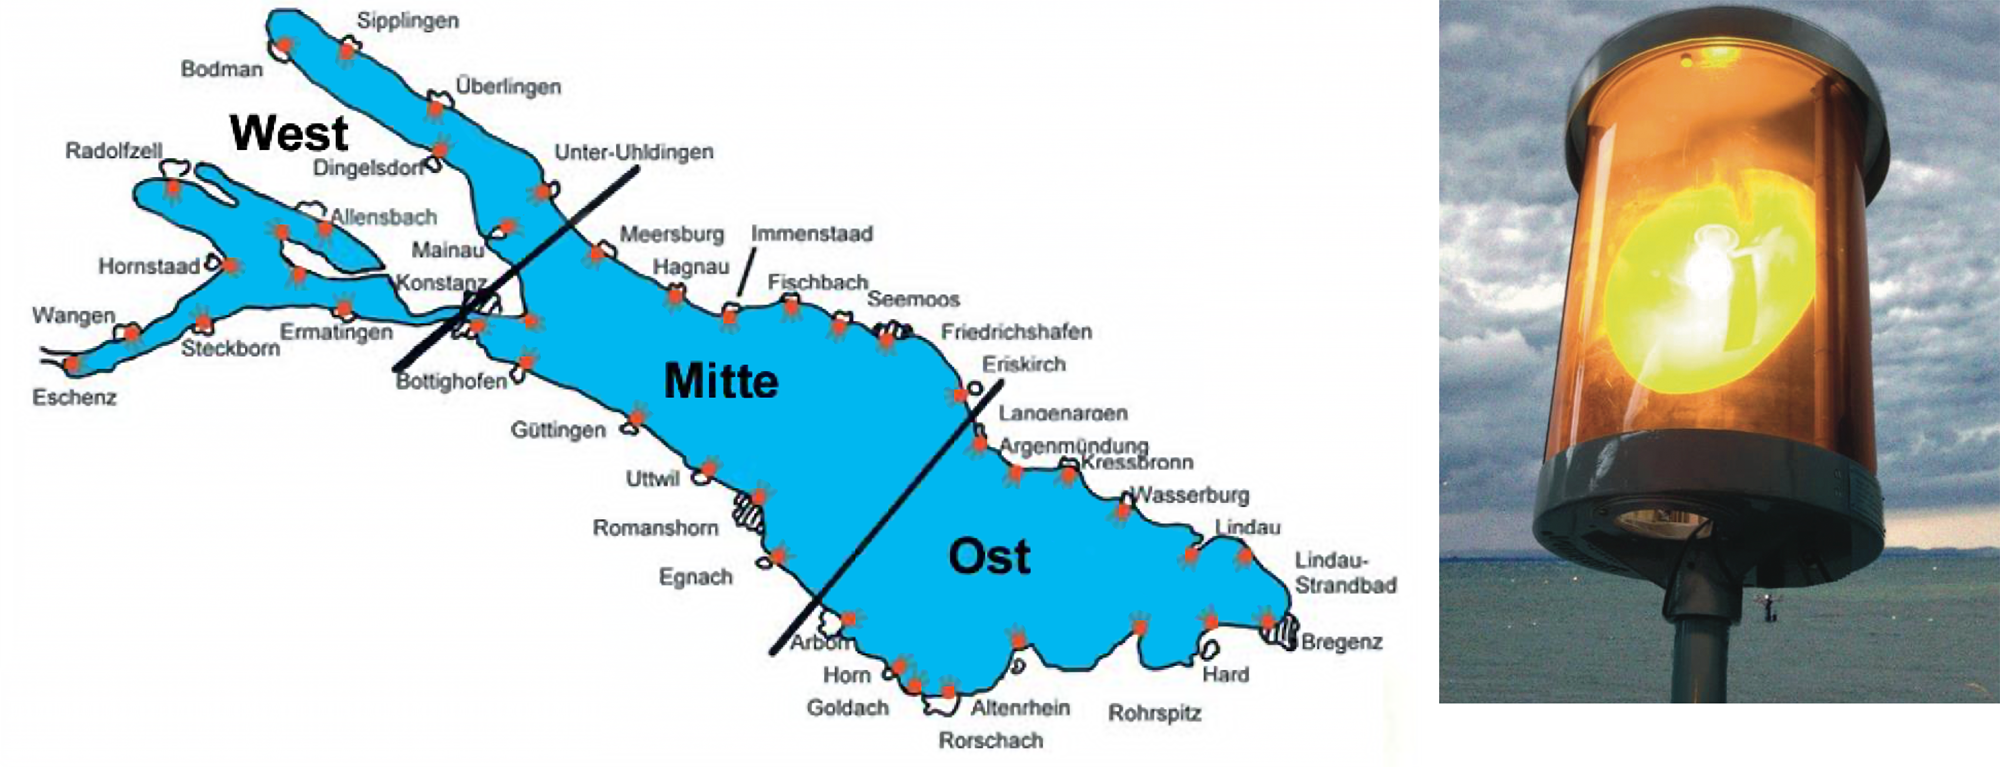
\includegraphics[width=\textwidth-2\fboxsep-2\fboxrule]{img/sturm2}}
	%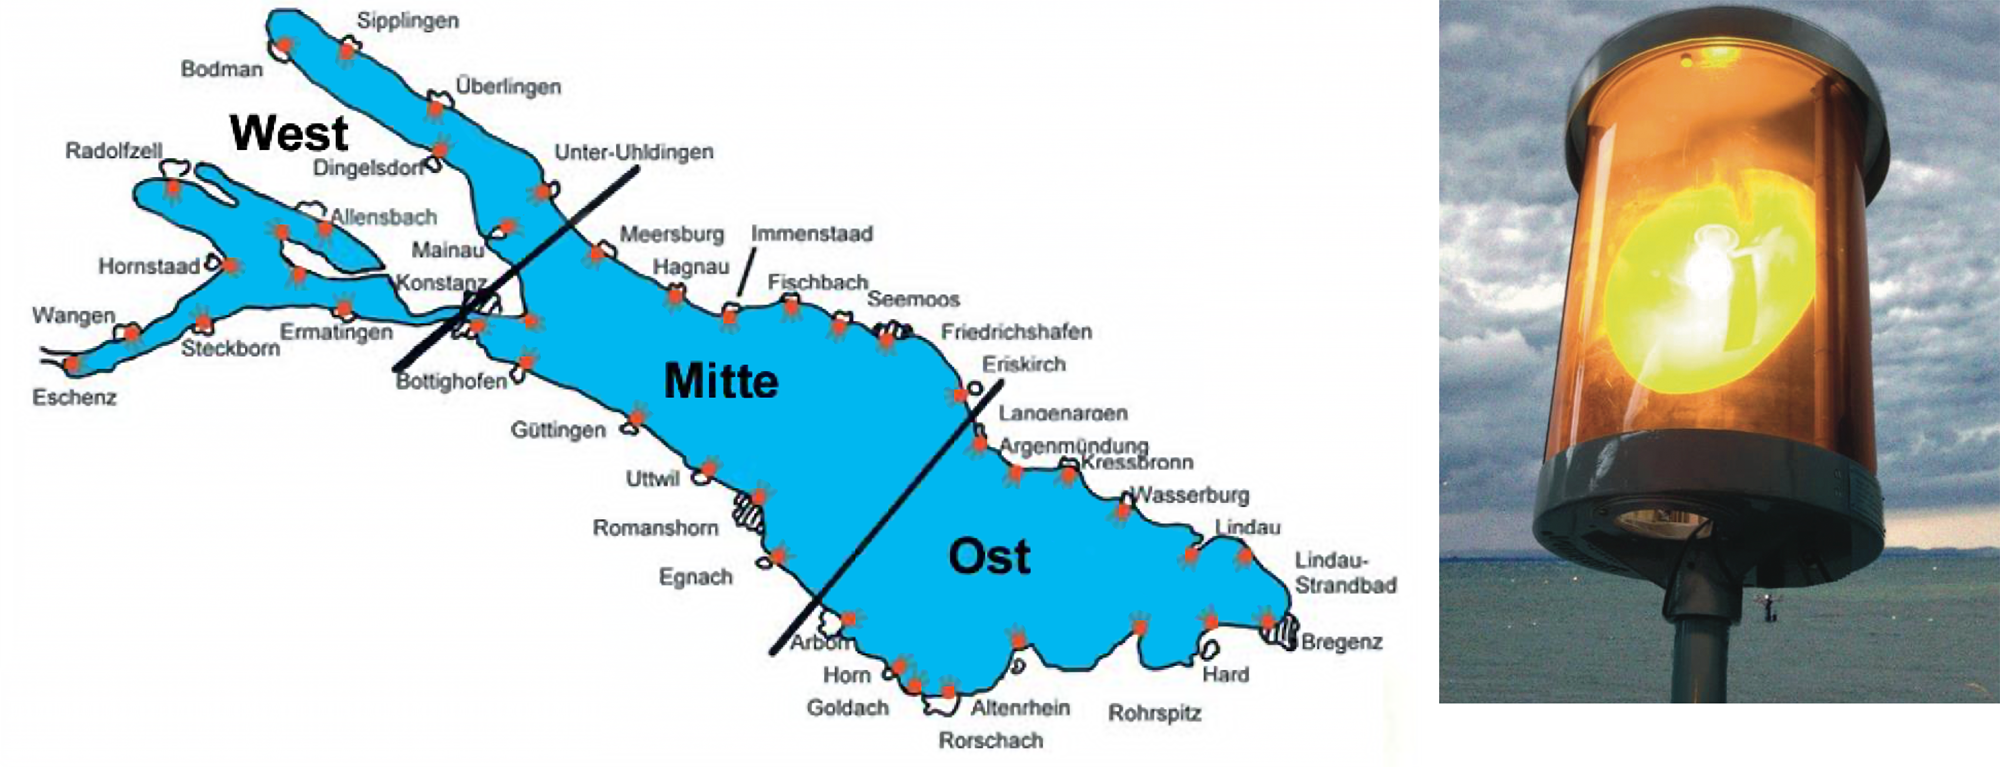
\includegraphics[width=1\linewidth]{img/sturm2}
	\caption{Sturmwarndienst Bodensee}
	\label{img:sturm2}
\end{figure}

% Problem: Kostenpflichtige Informaiton
Den aktuellen Status der Sturmwarnung kann sowohl beim Deutschen Wetterdienst, als auch bei meteoschweiz kostenpflichtig bezogen werden (ca. 1300CHF/Jahr). Kostenlos gibt es nur zwei browserkomatible Quellen: Das eine ist die allgemeine Mini-Warnkarte (173 x 109 Pixel) von meteoschweiz (siehe Abbildung \ref{img:sturm}, links) und das andere ist die Anzeige auf der Webseite der Kantonspolizei, Abbildung \ref{img:sturm}, rechts.

\begin{figure}[h!]
	\centering
  \fbox{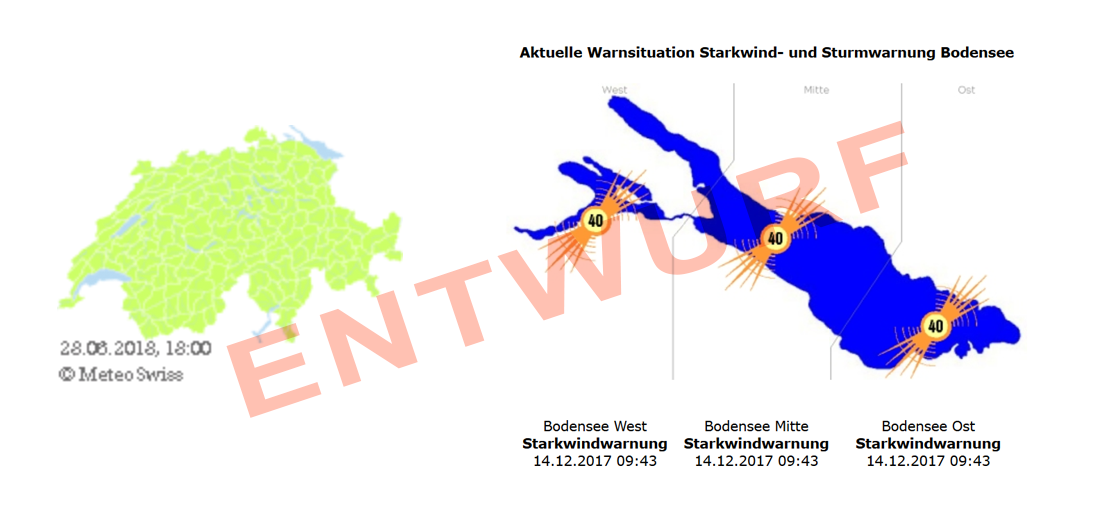
\includegraphics[width=\textwidth-2\fboxsep-2\fboxrule]{img/sturm}}
	%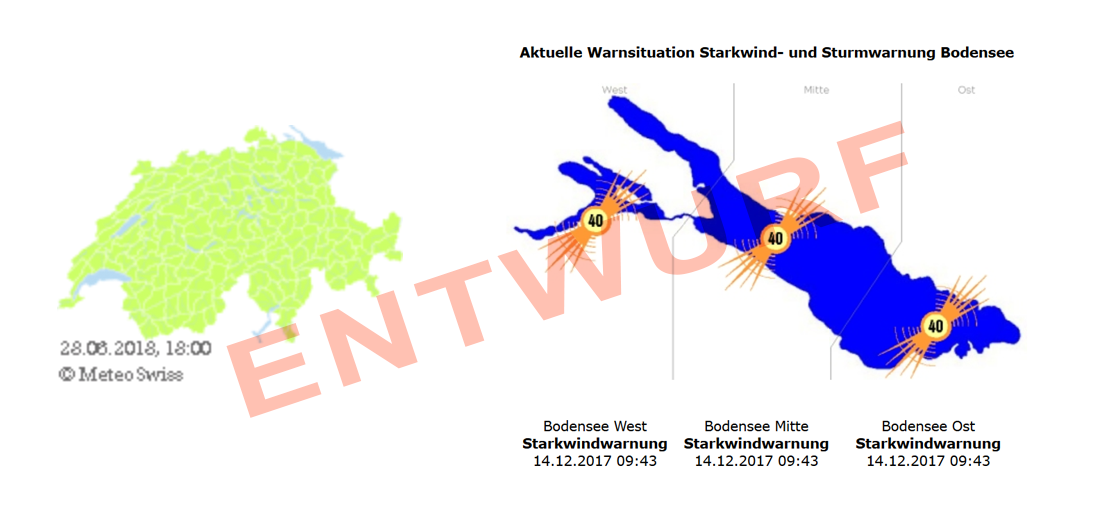
\includegraphics[width=1\linewidth]{img/sturm}
	\caption{Kostenlose Browserdarstellung}
	\label{img:sturm}
\end{figure}

Eine kostenlose API steht nicht zur Verfügung. Meteoschweiz verbietet es, Informaitonen von ihrer Website abzugreifen. Wir haben deshalb beim Amt für Informatik des Kantons Thurgau die Erlaubnis eingeholt, die Sturmwarndaten von der Kapo-Webseite abgreifen zu dürfen. Wir verwenden dazu die Python Bibliothek \textit{BeautifulSoup} als web crawler, wie in Listing \ref{lst:kttgCrawler} dargestellt. \newline

\begin{lstlisting}[label=lst:kttgCrawler,caption=Web Crawler für die Sturmwarndaten, language=python, style=py]
page = requests.get('http://www.kttg.ch/kapo/htm/stwarn.shtml')
soup = BeautifulSoup(page.text, 'html.parser')

# Einschaltzeit auslesen
soup.select('table tr:nth-of-type(4) td'):

# Status auslesen
soup.select('.titelfett strong'):
\end{lstlisting}

% Problem 1: keine API -> wenn Seite ändert, muss Crawler angepasst werden.
Das Problem beim Verwenden des Web Crawlers besteht darin, dass sobald die URL oder die Webseite geändert wird, der Crawler angepasst werden muss. Da der Crawler jedoch die einzige kostenlose Möglichkeit darstellt um die Daten zu erhalten, müssen wir dieses Risiko akzeptieren.

% Problem 2: Öffnungszeiten -> keine Warnung in der NAcht
Der Sturmwarndienst wie in Abschnitt \ref{subsec:sturmwarnung} beschrieben, ist kein 24h-Service. Der Dienst ist nur tagsüber aktiv zu den aufgelisteten Warnzeiten\footnote{ \url{https://kapo.tg.ch/public/upload/assets/56408/A5\%20Sturmwarnung.pdf}}, was aus Sicht der Sicherheit auf dem See nicht sehr sinnvoll ist.

\begin{itemize}
\item 1. April - 31. Oktober: 06:00 - 22:00 Uhr
\item 1. November - 31. März: 07:00 - 20:00 Uhr
\end{itemize}

\noindent
% Problem 3: rechtliche Verbindlichkeit der Sturmwarnung -> Zuverlässigkeit der anzeigen
Der Gedanke liegt nahe auf Grund der eigenen Windmessdaten eine Sturmwarnung anzuzeigen. In der Bodensee-Schifffahrts-Ordnung (BSO) Art. 6.13, steht jedoch:

\begin{quote}
\flqq Bereits bei Starkwind- und Sturmwarnung muss der Schiffsführer die durch die Umstände gebotenen Massnahmen treffen \frqq
\end{quote}

\noindent
 Da die Sturmwarnung auf dem Bodensee gesetzlche Pflichten mit sich bringt, haben wir uns entschlossen nur die offiziellen Daten anzuzeigen und nicht anderweitige Sturmwarnungen. Meteoschweiz bietet zudem auf ihrer MeteoSchweiz-App\footnote{ \url{https://www.meteoschweiz.admin.ch/home/service-und-publikationen/beratung-und-service/meteoschweiz-app.html}} die Möglichkeit von Push-Nachrichten bei Windwarnungen.




%-> Verweis auf Zeitungsartikel
%-> Meteoschweiz schickt in der Nacht keine SMS????? bzw. erstellt keine JSON????

% ins Kapitel API bzw. Cronjobs übernehmen
%Der Status der drei Teilabschnitte wird dann mintütlich in die Datenbank geschrieben. So kann der aktuelle Stand normal über die API abgefragt werden.

% nur im Vortrag erwähnen
% DAs JSON von Meteoschweiz kann leider nicht verwendet werden, da dessen URL bei jedem Update wechselt. Der genaue Pfad lässt sich nicht vorhersagen. Auf Grund des Zeitstempels lässt sich erahnen, dass es keine automatische Verbindung zwischen Meteoschweiz und den Sturmwarnleuchten am Bodensee gibt. Auf der Meteoschweiz-Seite ist z.B. der Zeitstempel 12:00 und auf der kttg.ch Seite 12:07. Wahrscheinlich erfolgt die Aktivierung manuell. Dies würde die Zeitdifferenz erklären.
% -> Foto Zeitstempel Meteoschweiz und kttg.ch
% Meteoschweiz leitet die Sturmwarnung an die Kantonspolizei Thurgau weiter. Diese schaltet die Sturmwarnung über eine eigne Software ein.








%% ###################################################################################################
%%   Unterkapitel
%% ###################################################################################################
\subsection{Darstellung der historischen Daten}

\subsubsection{Daten der alten Wetterstation}
\Diskussionspunkt{- sind unbrauchbar weil.....}\newline
\Diskussionspunkt{- Grafik der Daten auf Zeitschiene}\newline
\Diskussionspunkt{- Pegeldaten (Excel)}\newline

\subsubsection{Daten der neuen Wetterstation}
\Diskussionspunkt{- Printscreen ungefiltert}\newline
\Diskussionspunkt{- Printscreen gefiltert}\newline

Die historische Daten sollen möglichst interaktiv gestaltet sein und ein aussagekräftiges Bild des Wetterverhaltens aufzeigen. Die historischen Daten liegen als Stundenwerte in der Datebank vor.
Tableau Public \footnote{ \url{https://public.tableau.com/de-de/s/}} ist ein Visualisierungsprogramm, das die Möglichkeit bietet direkt auf die Datenbank zuzugreifen. Die Visualisierungen sind einfach zu erstellen und interaktiv vom Benutzer filterbar.
Tableu Public ist kostenlos mit der Einschränkung, dass sämtliche Visualisierungen öffentlich sind. In unserem Fall ist dies kein Problem, da wir die Visualisierungen sowieso veröffentlichen. Um Visualisierungen veröffentlichen zu können ist ein Account nötig. Die Visualisierung kann anschliessend in die eigene Webseite eingebettet werden.

Für die Auswertung haben wir uns auf die Lufttemperatur, die Windrichtung und -geschwindigkeit sowie den Regen konzentriert.
Der Vorteil von Tableau ist, dass die Visualisierungen sehr einfach angepasst werden können wenn z.B. neue Messdaten hinzukommen. Tableau bietet auch die Möglichkeit Darstellungen für verschiedene Display-Grössen anzulegen. Da der Benutzer selbst keine Eingaben machen kann, sondern nur Filter setzen, ist die Gefahr von SQL-Injektion nicht vorhanden.


\subsubsection{Tableau Public}
\Diskussionspunkt{- Filtermöglichkeiten}\newline

% Nachteil 1: Keine direkte Verbindung zur Datenbank
Tableau Public\footnote{ \url{https://public.tableau.com/de-de/s/}} ist kostenlos, bietet jedoch keine Möglichkeit live auf die Datenbank zuzugreifen. Die historischen Daten müssen demnach manuell periodisch auf den Tableau-Server kopiert werden.\newline

%Nachteil 2: Nicht responsive -> Workaround nötig
\Diskussionspunkt{- Mobile Darstellunbg}\newline
\Diskussionspunkt{- Printscreen der mobilen Darstellung}\newline
\Diskussionspunkt{- Codesniplet auswahl desktop oder mobile}\newline

% Nachteil 3: nicht barrierefrei
\Diskussionspunkt{- Barrierefreiheit? Farben}\newline
\Diskussionspunkt{- Barrierefreiheit? Semantisches Web}\newline





%% ###################################################################################################
%%   Unterkapitel
%% ###################################################################################################
\subsection{Automatische Aktualisierung der Anzeigeelemente}
\Diskussionspunkt{Initial Values beschreiben}\newline
Die Wetterstation erzeugt jede Minute einen Datenbank-Eintrag mit den aktuellen Messwerten. Damit eine geöffnete Webseite immer auf dem aktuellen Stand ist, wird eine poll-Funktion verwendet, die selbständig alle 61 Sekunden von der API die aktuellen Werte abfragt wie in \ref{lst:poll} verkürzt dargestellt. Sobald die JSON-Daten eingetroffen sind, wird die Funktion \textit{updateData} aufgerufen, die wiederum die Anzeigeelemente und Texfelder aktualisiert. Die gesamte Aktualisierung wird asynchron mittels AJAX durchgeführt. Die Seite wird dabei nicht neu geladen, nur die Anzeigewerte. \newline


\begin{lstlisting}[label=lst:poll,caption=Automatische Aktualisierung der Werte, language=JavaScript, style=htmlcssjs]
(function poll() {
        $.get('https://api.wetter-arbon.ch/v1/')
          .done(function(response) {updateData(response);})
          .always(function() {setTimeout(poll, 61000); });
})();

function updateData(res){
        pressure_gauge.refresh(res.v1.data.pressure.value);
        $("#cwassertemp1m") = res.v1.data.watertemperature1m.value;
}

\end{lstlisting}


%% ###################################################################################################
%%   Unterkapitel
%% ###################################################################################################
\subsection{Barrierefreier Zugang}
Die Wetterstation und ihre Webseite ist eine Dienstleistung der Stadt Arbon. Sie gehört der Bevölkerung und soll deshalb für möglichst alle zugänglich sein. Sowohl die \flqq Web Content Accessibility Guidelines\frqq\footnote{ \url{https://www.w3.org/TR/2008/REC-WCAG20-20081211/}} des W3C-Konsortiums, als auch die deutsche \flqq  Barrierefreie-Informationstechnik-Verordnung\frqq\footnote{ \url{https://www.gesetze-im-internet.de/bitv_2_0/BJNR184300011.html}} bieten diverse Inputs, wie die Bedienbarkeit und somit Zugänglichkeit einer Webseite verbesserte werden kann.
\newline

\noindent
%\subsection*{Problem}
WeatherDisplay Live, welches zum Anzeigen der Wetterdaten verwendet wird, ist eine proprietäre Software, die nur sehr eingeschränkt angepasst werden kann und auf Adobe Flash basiert. Es lassen sich beispielsweise die Anordnung der Anzeigeelemente und die Einheiten konfigurieren. Viel mehr nicht.  Adobe Flash gilt als kritische Technologie in Hinblick auf Barrierefreiheit. Mit der jetzigen Konfiguration können die Anforderung an eine barrierefreie Seite nicht umgesetzt werde.
\newline

\noindent
%\subsection*{Lösungsansatz}
Wie in Abschnitt \ref{subsec:flash} erläutert, muss WeatherDisplay Live ersetzt werden. Das bietet die Möglichkeit, dass die Entwicklung der neuen Webseite nach den oben erwähnten Richtlinien erfolgen kann.

Von einer verbesserten Zugänglichkeit profitieren nicht nur Menschen mit Einschränkungen. Es geht darum, die Webseite so zu gestalten, dass sie möglichst für alle Benutzergruppen zugänglich ist. Dazu zählen nicht nur Menschen mit Einschränkungen. Auch veraltete Technik oder aber der allerneueste Stand der Technik können zu Schwierigkeiten führen. Ein hoher Lärmpegel (z.B. in einer Fabrikhalle) oder der Zwang zur Stille (z.B. in einer Bibliothek), der keine akustische Ausgabe gestatten oder Lichtverhältnisse, die einen besonders hohen Kontrast erfordern beeinflussen die Bedienbarkeit einer Webseite. Eine von Microsoft beauftragte Studie~\cite{ForresterResearch2004E:Abilities} der \flqq Forrester Research Inc.\frqq schätzt, dass über 60 Prozent aller Computernutzer von Barrierefreiheit profitieren können und gemäss \flqq Interface Design\frqq ~\cite{ThesmannStephan2016ID:U} wird Barrierefreiheit bald Standard sein.

Die aktuellen Web Content Accessibility Guidelines\footnote{ \url{https://www.w3.org/TR/WCAG20/}} fordern die Einhaltung von vier Designprinzipien:

\begin{itemize}
\item Prinzip 1: Wahrnehmbarkeit
\item Prinzip 2: Bedienbarkeit
\item Prinzip 3: Verständlichkeit
\item Prinzip 4: Robustheit
\end{itemize}

Die Ziele dieser vier Prinzipien sind durch zwölf Richtlinien genauer spezifiziert.

% Zu jeder Richtlinie geben die WCAG2 testbare Erfolgskriterien (Success Criteria) vor.

% Priorität 1 („Muss-Kriterien“): Webauftritte müssen alle A-Anforderungen erfüllen, weil es sonst für eine oder mehrere Benutzergruppen unmöglich wäre, auf die Information im Dokument zuzugreifen.

% Priorität 2 („Soll-Kriterien“): Die Erfüllung der AA-Anforderungen beseitigt signifikante Hindernisse und erleichtert einer oder mehreren Benutzergruppen den Zugriff auf Web-Dokumente.

% Priorität 3 („Kann-Kriterien“): Diese AAA-Anforderungen können erfüllt werden, um den Zugriff auf Web-Dokumente für eine oder mehrere Benutzergruppen zu erleichtern. Sind die Prioritäten 1 bis 3 erfüllt, erhält das Informationsangebot die Konformitätsstufe AAA.


Daraus ergeben sich folgende relevante Anforderungen für die Webseite der Wetterstation:


\subsubsection*{Wahrnehmbarkeit}
% Anforderung 1.1: Text-Alternativen
% Anforderung 1.2: Zeitbasierte Medien -> nicht relevant
% Anforderung 1.3: Anpassbarkeit
% Anforderung 1.4: Unterscheidbarkeit
Alle Nicht-Text-Inhalte, die dem Benutzer präsentiert werden, haben eine Textalternative, die dem entsprechenden Zweck dient.
Für die Darstellung der Seite muss CSS verwendet werden. Die einzelenen Blöcke müssen sematisch korrekt bezeichnet werden (RL 1.3)
Alle Nicht-Text-Inhalte, die dem Benutzer präsentiert werden, haben eine Textalternative, die dem entsprechenden Zweck dient.
Farbe ist nicht das einzige visuelle Mittel, um Informationen zu vermitteln, eine Handlung anzuzeigen, eine Reaktion auszulösen oder ein visuelles Element zu unterscheiden. ext kann ohne Hilfsmittel bis zu 200 Prozent vergrössert werden, ohne dass der Inhalt oder die Funktionalität verloren geht. Die visuelle Darstellung von Text hat ein Kontrastverhältnis von mindestens 7:1.
Für die visuelle Darstellung von Textblöcken steht ein Mechanismus zur Verfügung, um folgendes zu erreichen: (Level AAA)
Vorder- und Hintergrundfarben können vom Anwender frei gewählt werden.
Die Breite beträgt nicht mehr als 80 Zeichen oder Glyphen (40 bei CJK).
Der Text ist links ausgerichtet
Der Zeilenabstand (Vorspann) ist innerhalb von Absätzen mindestens anderthalb mal so groß wie der Zeilenabstand, und der Absatzabstand ist mindestens 1,5 mal so groß wie der Zeilenabstand.
Die Größe des Textes kann ohne Hilfsmittel bis zu 200 Prozent verändert werden, ohne dass der Benutzer horizontal scrollen muss, um eine Textzeile in einem Vollbildfenster zu lesen.

Interessante Farb-Auswahlwerkzeuge:
Colorchecker\footnote{ \url{http://accessible-colors.com}}
Colorsave\footnote{ \url{http://colorsafe.co}}
Colorbrewer\footnote{ \url{http://colorbrewer2.org}}


Problematisch ist die Kombination von Komplementärfarben, weil sie zu Flimmern führen können.~\cite{HellbuschJanEric2011Bvuu}

\subsubsection*{Bedienbarkeit}
% Anforderung 2.1: Zugänglichkeit per Tastatur
% Anforderung 2.2: Bereitstellung ausreichender Zeit
% Anforderung 2.3: Vermeidung von Anfällen
% Anforderung 2.4: Navigierbarkeit
Alle Funktionen des Inhalts sind über eine Tastaturschnittstelle bedienbar.
Webseiten enthalten nichts, was in einer Sekunde mehr als dreimal blinkt.
Der Zweck eines jeden Links kann aus dem Linktext allein oder aus dem Linktext zusammen mit seinem programmatisch festgelegten Linkkontext bestimmt werden. Es gibt mehr als eine Möglichkeit, eine Webseite innerhalb einer Gruppe von Webseiten zu lokalisieren. Überschriften und Labels beschreiben das Thema oder den Zweck. Jede Tastatur bedienbare Benutzeroberfläche hat eine Betriebsart, bei der die Tastaturfokusanzeige sichtbar ist. Informationen über den Standort des Benutzers innerhalb einer Reihe von Webseiten sind verfügbar. Abschnittsüberschriften dienen der inhaltlichen Gliederung.



\subsubsection*{Verständlichkeit}
% Anforderung 3.1: Lesbarkeit
% Anforderung 3.2: Vorhersehbarkeit
% Anforderung 3.3: Hilfestellung bei der Eingabe

Die voreingestellte menschliche Sprache jeder Webseite kann programmgesteuert bestimmt werden. Die menschliche Sprache jeder Passage oder Phrase im Inhalt kann programmatisch bestimmt werden, mit Ausnahme von Eigennamen, Fachbegriffen, Wörtern unbestimmter Sprache und Wörtern oder Phrasen, die Teil der Umgangssprache des unmittelbar umgebenden Textes geworden sind. Ein Mechanismus zur Identifizierung der erweiterten Form oder Bedeutung von Abkürzungen steht zur Verfügung.  Wenn eine Komponente den Fokus erhält, löst sie keinen Kontextwechsel aus. Wenn ein Eingabefehler automatisch erkannt wird, wird das fehlerhafte Element identifiziert und der Fehler dem Benutzer in Textform beschrieben. Labels oder Anweisungen werden bereitgestellt, wenn der Inhalt eine Benutzereingabe erfordert.  Wird ein Eingabefehler automatisch erkannt und sind Korrekturvorschläge bekannt, so werden diese dem Anwender zur Verfügung gestellt.  Es steht eine kontextsensitive Hilfe zur Verfügung.



\subsubsection*{Robustheit}
% Anforderung 4.1: Kompatibilität
 In Inhalten, die mit Hilfe von Markup-Sprachen implementiert wurden, haben Elemente vollständige Start- und End-Tags, Elemente werden entsprechend ihrer Spezifikationen verschachtelt, Elemente enthalten keine doppelten Attribute und alle IDs sind eindeutig.




\subsubsection{Barrierefreie Grafiken}
\Diskussionspunkt{- Barrierefreiheit}\newline
